\documentclass{article}%
\usepackage[T1]{fontenc}%
\usepackage[utf8]{inputenc}%
\usepackage{lmodern}%
\usepackage{textcomp}%
\usepackage{lastpage}%
\usepackage[head=40pt,margin=0.5in,bottom=0.6in]{geometry}%
\usepackage{graphicx}%
%
\title{\textbf{Se inicia el cortejo fúnebre del concejal metropolitano fallecido Fernando Albán}}%
\author{EFE}%
\date{10/10/2018}%
%
\begin{document}%
\normalsize%
\maketitle%
\textbf{URL: }%
http://www.eluniversal.com/politica/22841/se{-}inicia{-}el{-}cortejo{-}funebre{-}del{-}concejal{-}metropolitano{-}fallecido{-}fernando{-}alban\newline%
%
\textbf{Periodico: }%
EU, %
ID: %
22841, %
Seccion: %
politica\newline%
%
\textbf{Palabras Claves: }%
NO\_TIENE\newline%
%
\textbf{Derecho: }%
1.1%
, Otros Derechos: %
1.2, 1.10%
, Sub Derechos: %
1.1.1.3, 1.2.2, 1.10.1%
\newline%
%
\textbf{EP: }%
SI\newline%
\newline%
%
\textbf{\textit{En la caminata, donde se observan cientos de personas con carteles que piden justicia y portan banderas de Venezuela, están presentes distintos dirigentes del partido opositor Primero Justicia}}%
\newline%
\newline%
%
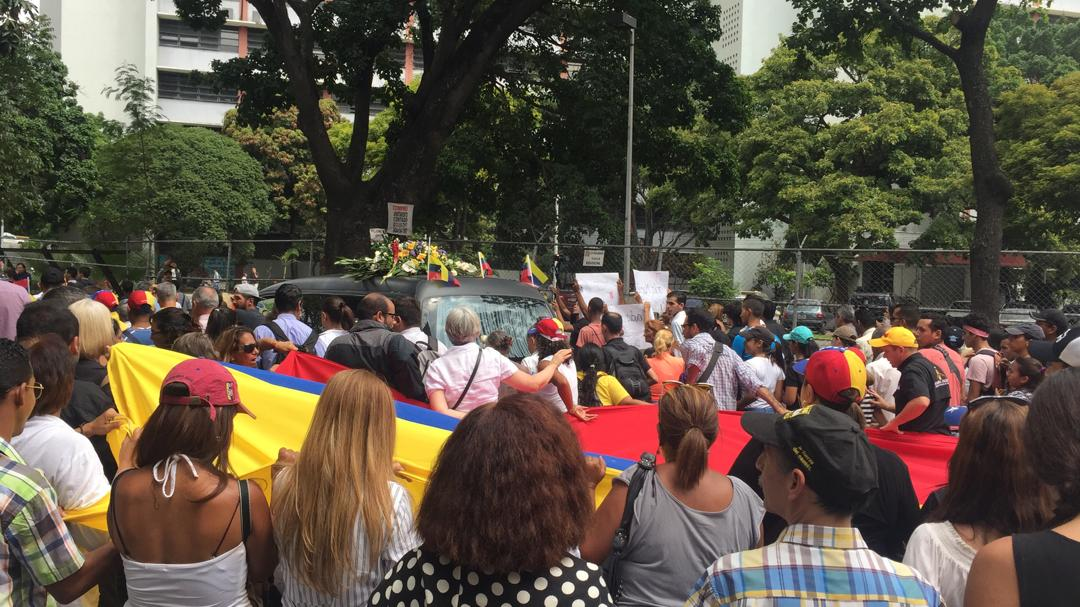
\includegraphics[width=300px]{253.jpg}%
\newline%
%
Caracas.{-}El cortejo fúnebre del concejal metropolitano fallecido Fernando Albán se inició este miércoles con una caminata y caravana que recorrerá más de doce kilómetros de la ciudad de Caracas para enterrar al político, que según la Fiscalía se suicidó, aunque opositores sostienen que se trata de un "asesinato".%
\newline%
%
La caminata y caravana comenzó cerca de las 11.00 de la mañana, luego de que se realizara una misa en la capilla de la Universidad Central de Venezuela (UCV), en el centro de la capital venezolana, y que fue oficiada por el cardenal Jorge Urosa Savino.%
\newline%
%
Albán, quien era concejal en el municipio caraqueño de Libertador y que fue detenido el viernes por supuestamente estar implicado en el atentado al presidente Nicolás Maduro, fue velado en esta capilla de la que era feligrés, según recordó el cardenal en esa homilía.%
\newline%
%
En la caminata, donde se observan cientos de personas con carteles que piden justicia y portan banderas de Venezuela, están presentes distintos dirigentes del partido opositor Primero Justicia (PJ){-} del que formaba parte Albán {-} como el dos veces candidato a la Presidencia, Henrique Capriles.%
\newline%
%
Además, hicieron acto de presencia otros dirigentes como la exdiputada María Corina Machado de Vente Venezuela, representantes del partido Voluntad Popular (VP) y diputados del Parlamento.%
\newline%
%
Los padres de Albán no han querido ofrecer declaraciones a la prensa y los miembros de PJ han pedido respeto para ellos.%
\newline%
%
Durante la misa, el cardenal Urosa reiteró que Albán estaba muy relacionado a la Iglesia católica venezolana y que servía a la Fundación Cáritas, así como en los programas que ha emprendido la institución religiosa para ayudar a los más necesitados en medio de la grave crisis económica que vive el país.%
\newline%
%
Los opositores han reiterado hoy su convencimiento de que el concejal fue "asesinado" y rechazan que se haya suicidado porque aseguran que tenía "profundos valores cristianos".%
\newline%
%
El opositor será enterrado en el Cementerio del Este de Caracas.%
\newline%
%
La Organización de las Naciones Unidas (ONU), la Unión Europea (UE), la Iglesia católica, partidos políticos, organizaciones de derechos humanos y varios Gobiernos han pedido al Ejecutivo de Nicolás Maduro una investigación independiente que determine responsabilidades en este caso.%
\newline%
%
\end{document}